\scanpage{24}
% letterhead
\noindent\begin{minipage}{0.66\textwidth}
\centering
I N S T I T U T\\
DES HAUTES ÉTUDES SCIENTIFIQUES\\
\rule{1cm}{0.4pt}
\end{minipage}

\handwritten{SGA 4 $\overline{\text{\uline{VII}}}$\quad p. 20}

\handwritten{%
% The three curved call lines are retained: the long line calls the upper
% addition before localement, and the two shorter lines call its reference
% and the reference after localement cohérent.  The terminal turn of the
% long line is not a comma following torsion.
\noindent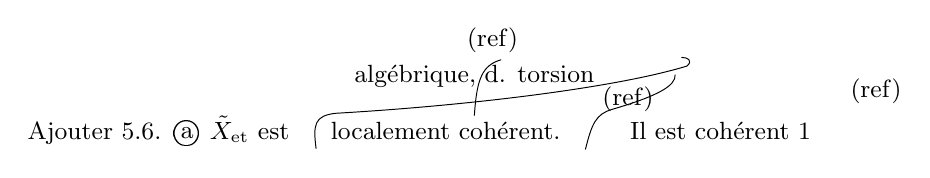
\begin{tikzpicture}[baseline=(a-prefix.base),x=1cm,y=1cm,inner sep=0pt,font=\small]
\node[anchor=base west] (a-prefix) at (0,0) {\uline{Ajouter} 5.6. \textcircled{a} $\tilde{X}_{\mathrm{et}}$ est};
\node[anchor=base west] (a-local) at (3.85,0) {localement cohérent.};
\node[anchor=base west] (a-il) at (7.65,0) {Il est cohérent \deleted{\illegible{1}}};
\node[anchor=base west] (a-add) at (4.15,.72) {\inserted{algébrique, d. torsion}};
\node[anchor=base west] (a-ref-one) at (5.58,1.18) {\inserted{(ref)}};
\node[anchor=base west] (a-ref-two) at (7.30,.43) {\inserted{(ref)}};
\node[anchor=base west] (a-ref-three) at (10.45,.53) {\inserted{(ref)}};
\draw[line width=.35pt] (3.67,-.12) .. controls (3.63,.19) and (3.65,.30) .. (3.92,.33)
  .. controls (5.65,.43) and (7.50,.66) .. (8.38,.93)
  .. controls (8.46,1.00) and (8.39,1.04) .. (8.31,1.04);
\draw[line width=.35pt] (5.68,.30) .. controls (5.71,.77) and (5.78,.94) .. (6.02,1.01);
\draw[line width=.35pt] (7.09,-.13) .. controls (7.17,.19) and (7.22,.32) .. (7.43,.38)
  .. controls (8.01,.55) and (8.24,.68) .. (8.23,.82);
\end{tikzpicture}
(resp. quasi-séparé\inserted{(ref)}) \deleted{\illegible{1}} sss le schéma $X$ est \deleted{\unsure{quasi-cpt|qu.-cpt}} cohérent i.e. qu. cpt qu. \unsure{sép|sep} (resp. quasi-séparé). \deleted{\illegible{1}}}

\handwritten{\textcircled{b} Soit $(X_i)_{i\in I}$ système projectif filtrant à morphismes de transition affines, $X=\varprojlim_i X_i$ (EGA $\overline{\text{\uline{IV}}}$ 8),}

\handwritten{Âlors}
% The corollary is at the right of the conclusion, above En déduire.
\margin{\handwritten{%
\hspace*{-2.2cm}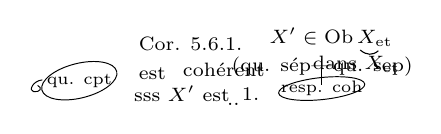
\begin{tikzpicture}[x=.01cm,y=.01cm,baseline=(cor-head.base),inner sep=0pt,font=\fontsize{7}{8}\selectfont]
\node[anchor=base west] (cor-head) at (132,-42) {\uline{Cor.} 5.6.1.};
\node[anchor=base west] (cor-ob) at (298,-34) {$X'\in\mathrm{Ob}\,X_{\mathrm{et}}$};
% Short curved stroke below the et of the first X, with no tilde above X.
\draw[line width=.4pt] (414,-42) .. controls (422,-49) and (430,-49) .. (437,-43);
\node[anchor=base west] at (132,-79) {est};
\node[anchor=base west] at (188,-76) {\deleted{\unsure{cohérent}}};
\node[anchor=base west] at (250,-69) {(\unsure{qu. sép|qu. sep})};
\node[anchor=base west] at (353,-67) {dans $X_{\mathrm{et}}$};
\node[font=\fontsize{6}{7}\selectfont] at (57,-81) {\inserted{qu. cpt}};
\draw[line width=.35pt,rotate around={14:(57,-81)}] (57,-81) ellipse [x radius=49,y radius=22];
\draw[line width=.35pt] (10,-80) .. controls (-2,-81) and (-8,-94) .. (-1,-95)
  .. controls (7,-96) and (11,-90) .. (4,-87);
\node[anchor=base west] at (126,-108) {sss $X'$ est};
\node[anchor=base west] at (244,-112) {..};
\node[anchor=base west] at (263,-106) {\deleted{\illegible{1}}.};
\node[font=\fontsize{6}{7}\selectfont] at (365,-91) {\inserted{resp. coh}};
\draw[line width=.35pt] (365,-54)--(365,-87);
\draw[line width=.35pt,rotate around={6:(365,-91)}] (365,-91) ellipse [x radius=55,y radius=14];
\end{tikzpicture}}}
\[
\handwritten{\tilde{X}_{\mathrm{et}}\simeq\underset{\longleftarrow}{\mathrm{limtop}}\,\tilde{X}_i.}
\]

\handwritten{En \unsure{deduire|déduire} pour 5.7.}

\figure{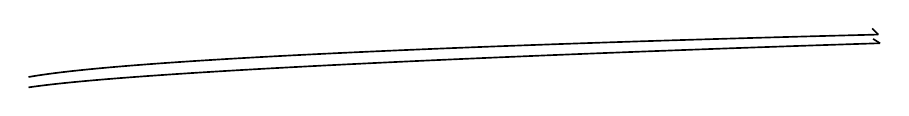
\begin{tikzpicture}[x=.011cm,y=.011cm]
\draw[line width=.6pt] (0,0) .. controls (140,25) and (700,42) .. (981,49);
\draw[line width=.6pt] (974,56)--(981,49);
\draw[line width=.6pt] (0,-12) .. controls (140,9) and (700,30) .. (983,39);
\draw[line width=.6pt] (975,44)--(983,39);
\end{tikzpicture}}

% Isolated faint bent stroke at the left of the pencil reference; function unknown.
\reversemarginpar
\margin{\begin{tikzpicture}[x=1mm,y=1mm]\draw[line width=.3pt] (0,0)--(.1,.7)--(.9,.5);\end{tikzpicture}}
\normalmarginpar
\handwritten{SGA 4 $\overline{\text{\uline{IX}}}$\quad p. 42\qquad note \uline{pour} la p. 8}
\figure{\begin{tikzpicture}[x=.012cm,y=.012cm]
\draw[line width=.4pt] (0,0) .. controls (270,25) and (489,51) .. (697,57)
  .. controls (814,61) and (920,63) .. (1000,67);
\end{tikzpicture}}

\handwritten{$\overline{\text{\uline{VII}}}$\quad 2.1 c)\qquad (p. 9)\quad \uline{corriger}}
% archive sheet number: 23
